\documentclass[twoside,10pt]{article}
\usepackage{amsmath,amsfonts,amsthm,fullpage,amssymb}
%\usepackage{mymath}
\usepackage{algorithm,amsmath,amssymb}
\usepackage{algorithmic}
\usepackage{graphicx, color}
\usepackage{url}

\usepackage{mdframed}
\usepackage{dsfont}
\usepackage{enumitem}
\usepackage{pdfpages}
\usepackage{amsmath,amsfonts,amsthm,fullpage,amssymb}
\usepackage{algorithm}
\usepackage{algorithmic}
\usepackage{graphicx}
\usepackage{url}
\usepackage{titling}
\usepackage[backend=biber,sorting=ynt]{biblatex}
\usepackage{tcolorbox}
\usepackage[colorlinks=true, hidelinks]{hyperref}
\hypersetup{
    colorlinks=true,
    linkcolor=blue,
    citecolor=blue,
}
\usepackage{listings}
\usepackage{xcolor}
\lstdefinestyle{mystyle}{
    backgroundcolor=\color{backcolour},   
    commentstyle=\color{codegreen},
    keywordstyle=\color{magenta},
    numberstyle=\tiny\color{codegray},
    stringstyle=\color{codepurple},
    basicstyle=\ttfamily\footnotesize,
    breakatwhitespace=false,         
    breaklines=true,                 
    captionpos=b,                    
    keepspaces=true,                 
    numbers=left,                    
    numbersep=5pt,                  
    showspaces=false,                
    showstringspaces=false,
    showtabs=false,                  
    tabsize=2
} 
\addbibresource{references.bib}
\setlength{\droptitle}{-3cm} % Moves the title up

\begin{document}


\title{ISYE 6740 Homework 5 \\ 
Fall 2025\\ 
Prof. Yao Xie\\
 Total 100 points}
 \author{Student Name Here}
\date{}
\maketitle



% \vspace{-.5cm}
\textbf{Provided Data and Submission Requirements:}
\begin{itemize}[noitemsep]
    \item All results, explanations, and math must be included in your PDF submission. Handwritten work is not accepted per the syllabus. Screenshots of work is also not accepted.
    \item If applicable, questions marked with \textbf{GS} must be submitted to Gradescope. Failure to pass gradescope tests will result in penalties to the points for that question.
\end{itemize}

\textbf{This assignment does not have any gradescope requirements}

\begin{itemize}[noitemsep]
    \item Q2: Comparing multi-class classifiers for MNIST Datasets [mnist\_10digits.mat, fashion-mnist\_train.csv, fashion-mnist\_test.csv]
    \item Q6: Medical imaging reconstruction [cs.mat]
\end{itemize}
As usual, please submit a report with sufficient explanation of your answers to each the questions, together with your code, in a zip folder.

\subsection*{1. Bayes classifier optimality. (10 points)}

Prove that the Bayes classifier is optimal in that it minimizes the Bayes risk. 
%
Let $X\in \mathbb R^d$ be a feature vector, and $Y\in \{1, 2, \ldots, K\}$ be the class label. Let $P(Y = k|X)$ be the posterior probability of class $k$ given the feature $X$. Let $h(X)$ be any classifier mapping $X$ to one of the class labels. Define the risk of the classifier as (the probability of mis-classification): \[R(h) = P(h(X)\neq Y).\] Then show that the Bayesian classifier $h^*$ (defined by picking the maximum posterior) achieves the minimum risk among all classifiers
\[h^*=\arg\min_h R(h)\]

\textit{\small 
Hint: Note that
\[R(h) = P(h(X)\neq Y) = 1-P(h(X) = Y)\]
Then note that 
\[P(h(X) = Y)= \mathbb E_{X} [\mathbb E_{Y|X} [\mathbb I\{h(X)= Y|X)\}]],\]
where the expectation is taken with respect to $X$, and the conditional expectation, respectively; and $\mathbb I$ denotes the indicator function. }


\subsection*{2. Comparing multi-class classifiers for MNIST Datasets. (10 points)}

This question will compare different classifiers and their performance for multi-class classifications on the complete MNIST dataset, looking at both MNIST\_Digits and MNIST\_Fashion. Use the data files provided in the homework folder. Both MNIST datasets have 60,000 training examples and 10,000 test examples. We will compare {\bf KNN, logistic regression, SVM, kernel SVM, and neural networks}. 

\begin{itemize}[noitemsep]

\item Use 6740 as your random\_state / random seed
\item You should standardize the data before training your classifiers by mapping the range from [0,255] to [0,1].

\item You will run your models on both MNIST\_DIGITS and MNIST\_FASHION. The shape of your data after loading should be as follows:
    \begin{itemize}
        \item xtrain (60000, 784)
        \item xtest (10000, 784)
        \item ytrain (60000,)
        \item ytest (10000,)
    \end{itemize}

\item load MNIST\_DIGITS using scipy.io.loadmat

\item Utilize the following models from sklearn: 
  \begin{itemize}
    \item LogisticRegression
    \item KNeighborsClassifier : Adjust K to obtain a reasonable result. Feel free to use any reasonable tuning methodology, only report your best K
    \item MLPClassifier : Use \textsf{hidden\_layer\_sizes = (20, 10)}
    \item SVC : Use this for both SVM and Kernel SVM. Randomly downsample the training data to size $m=5000$ for efficiency. For kernel SVM, use radial basis function kernel (rbf).
  \end{itemize}
\end{itemize}

Train the classifiers on the training dataset and evaluate them on the test dataset.

\begin{enumerate}

\item (5 points) Report the precision, recall, and F-1 score for each of the classifiers. The classification metrics should be reported for each class in the dataset. Provide these results for both the digits and fashion datasets.

 
\item (5 points) Discuss the performance of the classifiers. Include explanations both on comparing the 5 classifiers against each other for the individual datasets, and some insight into performance on the different datasets. Which model performed best on each dataset, and why might some models perform better than others?

 
\end{enumerate}


\subsection*{3. SVM (25 points).}

\begin{enumerate}
\item (5 points) Explain why can we set the margin $c = 1$ to derive the SVM formulation? Justify using a mathematical proof.
{\bf Answer 3.1}\\
The basic explanation of why we can set $c=1$ is because the scaler margin term can be absorbed into the $w$ and $b$ terms through scaling without impacting the maximization of the boundary. We've often manipulated scalers out of optimization equations because they do not affect the outcome. This is another such case. The decision boundary equation is:
\begin{align*}
    w^Tx + b &= 0
\end{align*}

A boundary that correctly classifies the data points with a margin $c$ between the boundary and the closest data points is:
\begin{align*}
    w^Tx + b &\geq c, \quad \text{for } y = 1 \\
    w^Tx + b &\leq -c, \quad \text{for } y = -1 \\
    \intertext{Simplify by adding the class label $y$} \\
    y(w^Tx + b) &\geq c
\end{align*}

We can use this to parameterize the boundary equation given two points:
\begin{align*}
    \tilde{\gamma} &= w^T(x^1 - x^2) = 2c \\
    \intertext{We can now normalize this margin with the L2 norm of $w$} \\
    \gamma &= \frac{2c}{\|w\|}
\end{align*}

The point of SVM is to find the boundary term that maximizes the margin $\gamma$ while also correctly classifying the data points.
\begin{align*}
    \max_{w,b} \gamma &= \frac{2c}{\|w\|} \quad \text{s.t. } y^i(w^Tx^i + b) \geq c, \forall i
\end{align*}

Now, the only impact of $c$ is to scale $w$ and $b$. So, if we just redefine those to incorporate the scaling, we can set $c=1$. 
\begin{align*}
    \text{Redefine } w = cw', &\quad b = cb' \\
    \intertext{Substituting these into the prior equations:} \\
    y(c (w'^Tx^i + b')) \geq c &\implies y(w^Tx^i + b) \geq 1 \\
    \gamma = \frac{2c}{c\|w'\|} &\implies \gamma = \frac{2}{\|w\|}
\end{align*}

At the end, we can just drop the 2 since it is a constant that does not impact the maximization to get the final formulation. We can also recognize that maximizing $\frac{1}{\|w\|}$ is the same as minimizing $\|w\|$. We can also square the norm to make it easier to solve.
\begin{align*}
    \max_{w,b} \gamma &= \frac{1}{\|w\|} \quad \text{s.t. } y^i(w^Tx^i + b) \geq 1, \forall i \\
    \text{Equivalently: } \quad \min_{w,b} \gamma &= \|w\|^2 \quad \text{s.t. } y^i(w^Tx^i + b) \geq 1, \forall i
\end{align*}

\item (5 points) Using Lagrangian dual formulation, show that the weight vector can be represented as
\[
w = \sum_{i=1}^n \alpha_i y_i x_i.
\]
where $\alpha_i \geq 0$ are the dual variables. What does this imply in terms of how to relate data to $w$?
{\bf Answer 3.2}\\
From the slides, we are given the dual primal formulation. We can take $\frac{\partial L}{\partial w}=0$ to find the optimal value.
\begin{align*}
    L(w,b,\alpha) &= \frac{1}{2} w^Tw + \sum_{i=1}^m \alpha_i(1-y^i(w^Tx^i + b)) \\
    \frac{\partial L}{\partial w} &= 0 = w - \sum_{i=1}^m \alpha_i y^ix^i \\
    w &= \sum_{i=1}^m \alpha_i y^ix^i \\
\end{align*}

Since $\alpha_iy^i$ is scalar, this means that the optimal $w$ is a linear combination of the data. 

\item (5 points) Explain why only the data points on the ``margin'' will contribute to the sum above, i.e., playing a role in defining $w$. Hint: use the Lagrangian multiplier derivation and KKT condition we discussed in class. 
{\bf Answer 3.3}\\
We will focus on the complementarity condition in the KKT functions:
\begin{align*}
    \alpha_i g_i(w) &= 0 \\
    \alpha_i(1-y^i(w^Tx^i + b)) = 0
\end{align*}
The condition above basically states that either $alpha_i$ or $(1-y^i(w^Tx^i + b))$ is zero.

Note that the internal function that is multiplied by $\alpha_i$ is the function describes the margin line. In the case that the data point is on the margin, then $1-y^i(w^Tx^i + b) = 0$. This means that $\alpha_i$ can be any value $\geq 0$. This means that the $\alpha_i$ for these points can be non-zero and contribute to the sum.

In the case that the data point is not on the margin, then $(1-y^i(w^Tx^i + b)) \neq 0$, so the $\alpha_i$ must be zero and thus it cannot contribute to the summation.

\item Simple SVM by hand. 

Suppose we only have four training examples in two dimensions as shown in Fig. The positive samples at $x_1 = (0, 0)$, $x_2 = (2, 2)$ and negative samples at $x_3 = (h, 1)$ and $x_4 = (0, 3)$. 
%
\begin{center}
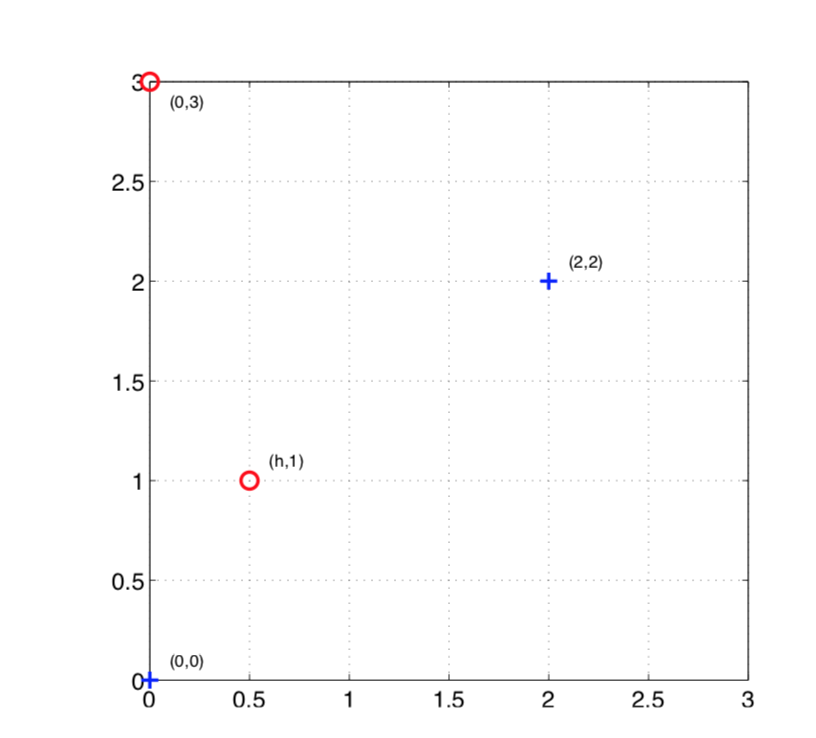
\includegraphics[width = 0.5\textwidth]{svm}
\end{center}

\begin{enumerate}
\item (5 points) For what range of parameter $h > 0$, the training points are still linearly separable? Be sure to consider all possible ranges.
\\{\bf Answer 3.4.a} \\
From the image, the decision boundary will be linearly separable as long as the line between $x_3$ and $x_4$ does not cross the line between $x_1$ and $x_2$.
The line between $x_1$ and $x_2$ has a slope of 1, so the equation of the line is $y = x$. The line between $x_3$ and $x_4$ has a slope of $\frac{3-1}{0-h} = \frac{2}{-h}$. The equation of this line is $y - 1 = \frac{2}{-h}(x - h)$, or $y = -\frac{2}{h}x + 3$.

From the image, we can see that two such scenarios exist:
\begin{itemize}
    \item The line between $x_3$ and $x_4$ is above and to the left of $y=x$. This happens if $0<h<1$.
    \item The line between $x_3$ and $x_4$ has a slope: $\frac{-1}{2} < slope < 0$. This happens if $h>4$.
\end{itemize}
\item (5 points) Does the orientation of the maximum margin decision boundary change as $h$ changes, when the points are separable? Please explain your conclusion.
\\ {\bf Answer 3.4.b} \\
Yes, the orientation of the maximum margin decision boundary does change as $h$ changes. Logically, the SVM boundary is determined by the support vectors. As $h$ changes, this can change the support vectors in a way that changes the boundary orientation. In the first case, the boundary will have a positive slope. In the second case, the boundary will have a negative slope.
\end{enumerate}


\end{enumerate}


\subsection*{4. Neural networks and backpropagation. (15 points)}


Consider a simple two-layer network in the lecture slides. Given $m$ training data $(x^i, y^i)$, $i = 1, \ldots, m$, the cost function used to training the neural networks
\[
\ell(w, \alpha, \beta) = \sum_{i=1}^m (y^i - \sigma(w^T z^i))^2
\]
where $\sigma (x) = 1/(1+e^{-x})$ is the sigmoid function, $z^i$ is a two-dimensional vector such that  $z_1^i = \sigma(\alpha^T x^i)$, and $z_2^i = \sigma(\beta^T x^i)$.
\\
Be sure to show all steps of your proofs.

\begin{enumerate}
\item (5 points) Show that the gradient is given by
\[
\frac{\partial \ell(w, \alpha, \beta) }{\partial w}
= - \sum_{i=1}^m 2(y^i - \sigma(u^i))\sigma(u^i)(1-\sigma(u^i)) z^i,
\]
where $u^i = w^T z^i$. 

{\bf Answer 4.1}\\
We can apply the chain rule for a single data point:
\begin{align*}
    u^i = w^Tz^i \quad &\Rightarrow \quad \frac{\partial u^i}{\partial w} = z^i \\
    b = \sigma(u^i) \quad &\Rightarrow \quad \frac{\partial b}{\partial u^i} = \sigma(u^i)(1-\sigma(u^i)) \\
    c = y^i-b \quad &\Rightarrow \quad \frac{\partial c}{\partial b} = -1 \\
    d = c^2 \quad &\Rightarrow \quad \frac{\partial d}{\partial c} = 2c \\
    \frac{\partial \ell(w, \alpha, \beta) }{\partial w} &= (\frac{\partial d}{\partial c})(\frac{\partial c}{\partial b})(\frac{\partial b}{\partial u^i})(\frac{\partial u^i}{\partial w})\\
    \frac{\partial \ell(w, \alpha, \beta) }{\partial w} &= [2(y^i-\sigma(u^i))][-1][(\sigma(u^i))(1-\sigma(u^i))][z^i]
\end{align*}

Simplify and sum over all data points:
\begin{align*}
    \frac{\partial \ell(w, \alpha, \beta) }{\partial w} = - \sum_{i=1}^m 2(y^i - \sigma(u^i))\sigma(u^i)(1-\sigma(u^i)) z^i
\end{align*}


\item (10 points) Also, show the gradient of $\ell(w, \alpha, \beta)$ with respect to $\alpha$ and $\beta$ and write down their expression.
{\bf Answer 4.2}\\
{\bf Gradient w.r.t. $\alpha$:}
We can apply the chain rule for a single data point:
\begin{align*}
    f^i = \alpha^T x^i \quad &\Rightarrow \quad \frac{\partial f^i}{\partial \alpha} = x^i \\
    z_1^i = \sigma(f^i) \quad &\Rightarrow \quad \frac{\partial z_1^i}{\partial f^i} = (\sigma(f^i))(1-\sigma(f^i)) \\
    u^i = w_1z_1^i + w_2z_2^i \quad &\Rightarrow \quad \frac{\partial u^i}{\partial z_1^i} = w_1 \\
    b = \sigma(u^i) \quad &\Rightarrow \quad \frac{\partial b}{\partial u^i} = \sigma(u^i)(1-\sigma(u^i)) \\
    c = y^i-b \quad &\Rightarrow \quad \frac{\partial c}{\partial b} = -1 \\
    d = c^2 \quad &\Rightarrow \quad \frac{\partial d}{\partial c} = 2c \\
    \frac{\partial \ell(w, \alpha, \beta) }{\partial \alpha} &= (\frac{\partial d}{\partial c})(\frac{\partial c}{\partial b})(\frac{\partial b}{\partial u^i})(\frac{\partial u^i}{\partial z_1^i})(\frac{\partial z_1^i}{\partial f^i})(\frac{\partial f^i}{\partial \alpha})\\
    \frac{\partial \ell(w, \alpha, \beta) }{\partial \alpha} &= [2(y^i-\sigma(u^i))][-1][(\sigma(u^i))(1-\sigma(u^i))][w_1][(\sigma(\alpha^T x^i))(1-\sigma(\alpha^T x^i))][x^i]
\end{align*}

Simplify and sum over all data points:
\begin{align*}
    \frac{\partial \ell(w, \alpha, \beta) }{\partial \alpha} = - \sum_{i=1}^m 2[y^i-\sigma(u^i)][(\sigma(u^i))(1-\sigma(u^i))][w_1][(\sigma(\alpha^T x^i))(1-\sigma(\alpha^T x^i))][x^i]
\end{align*}
{\bf Gradient w.r.t. $\beta$:}
We can apply the chain rule for a single data point:
\begin{align*}
    g^i = \beta^T x^i \quad &\Rightarrow \quad \frac{\partial g^i}{\partial \beta} = x^i \\
    z_2^i = \sigma(g^i) \quad &\Rightarrow \quad \frac{\partial z_2^i}{\partial g^i} = (\sigma(g^i))(1-\sigma(g^i)) \\
    u^i = w_1z_1^i + w_2z_2^i \quad &\Rightarrow \quad \frac{\partial u^i}{\partial z_2^i} = w_2 \\
    b = \sigma(u^i) \quad &\Rightarrow \quad \frac{\partial b}{\partial u^i} = \sigma(u^i)(1-\sigma(u^i)) \\
    c = y^i-b \quad &\Rightarrow \quad \frac{\partial c}{\partial b} = -1 \\
    d = c^2 \quad &\Rightarrow \quad \frac{\partial d}{\partial c} = 2c \\
    \frac{\partial \ell(w, \alpha, \beta) }{\partial \beta} &= (\frac{\partial d}{\partial c})(\frac{\partial c}{\partial b})(\frac{\partial b}{\partial u^i})(\frac{\partial u^i}{\partial z_2^i})(\frac{\partial z_2^i}{\partial g^i})(\frac{\partial g^i}{\partial \beta})\\
    \frac{\partial \ell(w, \alpha, \beta) }{\partial \beta} &= [2(y^i-\sigma(u^i))][-1][(\sigma(u^i))(1-\sigma(u^i))][w_2][(\sigma(\beta^T x^i))(1-\sigma(\beta^T x^i))][x^i]
\end{align*}

Simplify and sum over all data points:
\begin{align*}
    \frac{\partial \ell(w, \alpha, \beta) }{\partial \beta} = - \sum_{i=1}^m 2[y^i-\sigma(u^i)][(\sigma(u^i))(1-\sigma(u^i))][w_2][(\sigma(\beta^T x^i))(1-\sigma(\beta^T x^i))][x^i]
\end{align*}
\end{enumerate}


\subsection*{5. Feature selection and change-point detection. (20 points)} 

\begin{enumerate}

\item (10 points) Consider the mutual information-based feature selection. Suppose we have the following table (the entries in the table indicate counts) for the spam versus and non-spam emails:
%
\begin{center}
\begin{tabular}{c|c|c|c}
\hline
$N=16860$ & ``prize'' = 1 & ``prize'' = 0 &\\\hline
``spam'' = 1 & $N_{11} = 145$& $N_{10} = 15$ & $N_{1.} = 160$\\ \hline 
 ``spam'' = 0 & $N_{01} = 1200$ & $N_{00} = 15500$ & $N_{0.} = 16700$\\\hline
 & $N_{.1} = 1345$ & $N_{.0} = 15515$ & \\ \hline
\end{tabular}
\end{center}

\begin{center}
\begin{tabular}{c|c|c|c}
\hline
$N=19190$ & ``hello'' = 1 & ``hello'' = 0 &\\\hline
``spam'' = 1 & $N_{11} = 160$ & $N_{10} = 30$ & $N_{1.} = 190$\\ \hline 
 ``spam'' = 0 & $N_{01} = 12500$ & $N_{00} = 6500$  & $N_{0.} = 19000$\\\hline
 & $N_{.1} = 12660$ & $N_{.0} = 6530$ & \\ \hline
\end{tabular}
\end{center}

Given the two tables above, calculate the mutual information for the two keywords, ``prize`` and ``hello'' respectively. Which keyword is more informative for deciding whether or not the email is spam? If any tools are used for your calculation, you must still show your mathematical steps in your report and include code/files used for your calculations.
\\{\bf Answer 5.1} \\
I modified the above tables to contain the relevant summations for the mutual information calculation. Calculating the mutual information answers the question: how much uncertainty about the class label is resolved by knowing the feature value. A higher mutual information result indicates that the feature is more informative about the label. Using the example from slide 17 in the feature selection lecture, we can calculate for both tables.
\begin{align*}
\intertext{\bf Prize table:} \\
I(U;C) &= \frac{N_{11}}{N} \log_2 \frac{N N_{11}}{N_{1.} N_{.1}} + 
    \frac{N_{01}}{N} \log_2 \frac{N N_{01}}{N_{0.} N_{.1}} +
    \frac{N_{10}}{N} \log_2 \frac{N N_{10}}{N_{1.} N_{.0}} +
    \frac{N_{00}}{N} \log_2 \frac{N N_{00}}{N_{0.} N_{.0}} \\
 &= 0.0278 \quad \text{(Calculation in submitted Python notebook)}
\end{align*}

\begin{align*}
\intertext{\bf Hello table:} \\
I(U;C) &= \frac{N_{11}}{N} \log_2 \frac{N N_{11}}{N_{1.} N_{.1}} + 
    \frac{N_{01}}{N} \log_2 \frac{N N_{01}}{N_{0.} N_{.1}} +
    \frac{N_{10}}{N} \log_2 \frac{N N_{10}}{N_{1.} N_{.0}} +
    \frac{N_{00}}{N} \log_2 \frac{N N_{00}}{N_{0.} N_{.0}} \\
     &= 0.0012 \quad \text{(Calculation in submitted Python notebook)}
\end{align*}
Judging from these results, the ``prize'' word is clearly more informative about whether or not an email is spam.

\item  (10 points)  Given two distributions, $f_0 = \mathcal{N}(0, 1)$, $f_1 = \mathcal{N}(0, 1.4)$, derive what should be the CUSUM statistic (i.e., show the mathematical CUSUM detection statistic specific to these distributions). Plot the CUSUM statistic for a sequence of 150 randomly generated i.i.d. (independent and identically distributed) samples, $x_1, \ldots, x_{100}$ according to $f_0$ and $x_{101}, \ldots, x_{150}$ according to $f_1$. Using your plot, please provide a reasonable estimation of where a change may be detected.\\
\textbf{Note: Be certain to set your random seed to 6740 to ensure reproducible results. Failure to do so will result in point deductions}


\end{enumerate}


\subsection*{6. Medical imaging reconstruction (20 points).} 

In this problem, you will consider an example resembles medical imaging reconstruction in MRI.  We begin with a true image image of dimension 50 $\times$ 50 (i.e., there are 2500 pixels in total). Data is \textsf{cs.mat}; you can plot it first. This image is truly sparse, in the sense that 2084 of its pixels have a value of 0, while 416 pixels have a value of 1. You can think of this image as a toy version of an MRI image that we are interested in collecting.

Because of the nature of the machine that collects the MRI image, it takes a long time to measure each pixel value individually, but it's faster to measure a linear combination of pixel values. We measure $n$ = 1300 linear combinations, with the weights in the linear combination being random, in fact, independently distributed as $\mathcal{N}(0,1)$. Because the machine is not perfect, we don't get to observe this directly, but we observe a noisy version. These measurements are given by the entries of the vector
\[
y = A x + \epsilon,
\]
where $y \in \mathbb R^{1300}$, $A \in \mathbb R^{1300\times 2500}$, and $\epsilon \sim \mathcal N(0, 25\times I_{1300})$ where $I_n$ denotes the identity matrix of size $n\times n$. In this homework, you can generate the data $y$ using this model. 

Now the question is: can we model $y$ as a linear combination of the columns of $x$ to recover some coefficient vector that is close to the image? Roughly speaking, the answer is yes. 

Key points here: although the number of measurements $n$ = 1300 is smaller than the dimension $p$ = 2500, the true image is sparse. Thus we can recover the sparse image using few measurements exploiting its structure. This is the idea behind the field of \textit{compressed sensing}. 

The image recovery can be done using lasso
\[
\min_x \|y-Ax\|_2^2 + \lambda \|x\|_1.
\]
\begin{enumerate}
\item (10 points) Now use lasso to recover the image and select $\lambda$ using 10-fold cross-validation. Plot the cross-validation error curves, and show the recovered image using your selected lambda values.

\item (10 points) To compare, also use ridge regression to recover the image:
\[
\min_x \|y-Ax\|_2^2 + \lambda \|x\|_2^2.
\]
Select $\lambda$ using 10-fold cross-validation. Plot the cross-validation error curves, and show the recovered image using your selected lambda values. Which approach gives a better recovered image?
\end{enumerate}



\end{document}
